\documentclass[]{beamer}
\newcommand{\argmin}{\operatornamewithlimits{argmin}}
\usepackage{hyperref}
\usepackage{amsmath} 
\usepackage{beamerthemesplit} 

\title{Data Mining \& Machine Learning}  
\subtitle{Regularization Methods for Regression}
\author{Francisco Javier Arceo \\
        Senior Data Scientist}
\institute{NYU Polytechnic School of Engineering \\ Commonwealth Bank of Australia}
\date{March 23, 2015}

\begin{document}
\begin{frame}
\titlepage
\end{frame}
\note{Talk for 30 minutes} % Add notes to yourself that will be displayed when
% typeset with the notes or notesonly class options

\section[Regularization Methods for Regression]{}
\begin{frame}
\tableofcontents
\end{frame}

% Slide 1
\section{L2 Norm: Ridge}
\subsection{Motivation}
\begin{frame}
\frametitle{Ridge Regression}   % Insert frame title between curly braces
\begin{equation}
\hat{\beta}_{ridge} = \argmin_{\beta} \sum_{i=1}^{n} (y_{i} - \sum_{j=1}^{p}\beta_{j}x_{ij})^2 + \lambda \sum_{j=1}^{p}\beta_{j}^2
\end{equation}
\begin{equation}
\boldsymbol{\hat{\beta}}_{ridge} = \argmin_{\beta} (\boldsymbol{y - x}^{T} \boldsymbol{\beta})^2 + \boldsymbol{\lambda \beta}^2
\end{equation}
\begin{itemize}
\item<1-> First published by the Russian Mathematician Andrey Nikolayevich Tikhonov (1906-1993) in 1943 % Use Next Page to go to Point 2
\item<2-> Originally called Tikhonov regularization % Use Next Page to go to Point 3
\item<3-> First introduced to the statistical literature in 1970 by Hoerl and Kennard (\emph{Technometrics})
\item<4-> Method to deal with non-invertible \pmb{(X'X)} matrices
                                                   \end{itemize}
                                                   \end{frame}
                                                   
                                                   % Slide 2
                                                   \subsection{Framework}
                                                   \begin{frame}
                                                   \frametitle{Ridge Regression}   % Insert frame title between curly braces
                                                   \begin{equation}
                                                   \hat{\beta}_{j,ridge} = \frac{\sum_{i=1}^{n} (x_{ij} - \bar{x_j})(y_i - \bar{y})} {\sum_{i=1}^{n} (x_{ij} - \bar{x_j})^2} \frac{1}{1+\lambda} = \frac{\hat{\beta}_{j,ols}} {1 + \lambda}
                                                   \end{equation}
                                                   \begin{equation}
                                                   \boldsymbol{\hat{\beta}}_{ridge} = \boldsymbol{ (X'X+\lambda I)^{-1} X'y}
                                                  \end{equation}
                                                  \begin{itemize}
                                                  \item<1-> Equation (3) is a special case of an orthonormal design matrix 
                                                  \item<2-> $\lambda$ is a penalty term that is added to the diagonal elements of $\boldsymbol{(X'X)}$ and $\boldsymbol{I}$ is an (nxn) matrix
\item<3-> Question: what happens when $\lambda$=0?
\item<4-> Back to Ordinary Least-Squares solution!
  \end{itemize}
\end{frame}

% Slide 3
\subsection{Similarities}
\begin{frame}
\frametitle{Ridge Regression}   % Insert frame title between curly braces
\begin{equation}
\boldsymbol{\hat{\beta}}_{ridge} = \argmin_{\beta} (\boldsymbol{y - x}^{T} \boldsymbol{\beta})^2 + \boldsymbol{\lambda \beta}^2
\end{equation}
\begin{equation}
\boldsymbol{\hat{\beta}}_{ridge} = \argmin_{\beta}( \sum_{i=1}^{n} (y_i-x_{i}^T \boldsymbol{\beta})^2) \hspace{0.2cm} s.t. ||\boldsymbol{\beta}||_2 \le t
\end{equation}
\begin{itemize}
\item<1-> Equation (5) is equivalent to solving the constrained optimization problem in equation (6)
\item<2-> Note that the $||\boldsymbol{\beta}||_2$ is the 2-norm of the vector $\boldsymbol{\beta}$ and $t \ge 0$
  \item<3-> What happens when we change the norm? What about the L1 norm?
\end{itemize}
\end{frame}

% Slide 4
\section{L1 Norm: Lasso}
\subsection{Similarities}
\begin{frame}
\frametitle{LASSO Regression}   % Insert frame title between curly braces
\begin{equation}
\boldsymbol{\hat{\beta}}_{ridge} = \argmin_{\beta}( \sum_{i=1}^{n} (y_i-x_{i}^T \boldsymbol{\beta})^2) \hspace{0.2cm} s.t. ||\boldsymbol{\beta}||_2 \le t
\end{equation}
\begin{equation}
\boldsymbol{\hat{\beta}}_{lasso} = \argmin_{\beta}( \sum_{i=1}^{n} (y_i-x_{i}^T \boldsymbol{\beta})^2) \hspace{0.2cm} s.t. ||\boldsymbol{\beta}||_1 \le t
\end{equation}
\begin{itemize}
\item<1-> $||\boldsymbol{\beta}||_1 = \sum_{j=1}^{p}|\beta_j|$, $||\boldsymbol{\beta}||_2 = \sum_{j=1}^{p}\beta_j^2$, and $p:=$ the number of features
\item<2-> $||\boldsymbol{\beta}||_1$ is the unit-norm of the vector $\boldsymbol{\beta}$ and $t \ge 0$ 
  \item<3-> Difference is in the constraint of the minimization problem
\end{itemize}
\end{frame}

% Slide 5
\subsection{Motivation}
\begin{frame}
\frametitle{LASSO Regression}   % Insert frame title between curly braces
\begin{equation}
\boldsymbol{\hat{\beta}}_{lasso} = \argmin_{\beta}( \sum_{i=1}^{n} (y_i-x_{i}^T \boldsymbol{\beta})^2) \hspace{0.2cm} s.t. ||\boldsymbol{\beta}||_1 \le t
\end{equation}
\begin{equation}
\boldsymbol{\hat{\beta}}_{lasso} = \argmin_{\beta} (\boldsymbol{y - x}^{T} \boldsymbol{\beta})^2 + \boldsymbol{\lambda |\beta|}
\end{equation}

\begin{itemize}
\item<1-> Equation (9) and (10) lead to a minimization similar to equation (2) from Ridge, except the penalization to $\beta$ is linear instead of quadratic
\item<2-> What's the benefit of using the L1-norm versus the L2-norm?
\item<3-> Sparsity!
\item<4-> Using LASSO results in models with less parameters (features)
\end{itemize}
\end{frame}

\subsection{Framework}
\begin{frame}
\frametitle{LASSO Regression}   % Insert frame title between curly braces
\begin{equation}
\boldsymbol{\hat{\beta}}_{lasso}(\lambda) = S(\hat{\beta},\lambda) \equiv sign(\hat{\beta})(|\hat{\beta}|-\lambda)_+ 
\end{equation}
\[
S(\hat{\beta},\lambda) =\begin{cases}
\hat{\beta} -  \lambda, \hspace{0.2cm} if \hat{\beta} > 0 \hspace{0.1cm} and \hspace{0.1cm} \lambda < | \hat{\beta} | \\
\hat{\beta} + \lambda, \hspace{0.2cm} if \hat{\beta} < 0 \hspace{0.1cm}and \hspace{0.1cm} \lambda < |\hat{\beta}| \\
0, \hspace{0.9cm} if  \lambda > |\hat{\beta} |.
\end{cases}
\]
\begin{equation}
\hat{\beta}_{j,lasso}^{t} \leftarrow S( \hat{\beta}_{j,lasso}^{t-1} +  \sum_{i=1}^{n} x_{ij} (y_i - \hat{y_{i}}^{t-1}), \lambda)
\end{equation}
\begin{itemize}
\item<1-> Equation (11) is called the soft-threshold operator 
\item<2-> Apply soft-threshold operator as we cycle through our features at the $t^{th}$ iteration (12) updating the residual along the way
\item<3-> LASSO does variable selection by setting select variables to 0!
\end{itemize}
\end{frame}

\section{Regularization Methods}
\subsection{Important Facts}
\begin{frame}
\frametitle{LASSO and Ridge Regression}   % Insert frame title between curly braces
\begin{itemize}
\item<1-> How do we choose $\lambda$? \bf{Cross Validation}
\item<2-> When do we use Ridge vs LASSO? When we want a model with less coefficients (predictors) use LASSO
\item<3-> LASSO can be used when p $>>$ n 
\item<4-> Both methods reduce the size of the coefficients but Ridge shrinks to 0 continuously; LASSO shrinks discretely
\item<5-> Both biased in the statistical sense but asymptotically unbiased and can be shown that they select the true features with probability $\rightarrow$  1
\end{itemize}
\end{frame}

\begin{frame}
\frametitle{LASSO and Ridge Regression}   % Insert frame title between curly braces
\begin{itemize}
\item<1-> Ridge and Lasso can be developed using a Bayesian framework
\item<2-> Equivalent to setting a Gaussian Prior and Laplace prior on each coefficient for Ridge and Lasso, respectively
\item<3-> Both are convex optimization problems where Ridge has a closed form solution and LASSO must be solved iteratively
\item<4-> L1 and L2-Norm can be extended to L-P Norm
\item<5-> P-norms $<$ 1 yield sparser models
\item<6-> Many different ways to regularize parameters, extensive literature exists
\item<7-> Useful in banking, tech, insurance, marketing, and other fields
\end{itemize}
\end{frame}

% New Slide
\subsection{Empirical Example: Kaggle's Amazon Competition}
\begin{frame}
\frametitle{LASSO and Ridge Regression}
\begin{itemize}
\item<1-> Amazon Kaggle competition: Employee Access Challenge
\item<2-> Training data on 32,768 employee with 
\item<3-> Outcome/Label is binary outcome of whether an employee received access (Average Training Response = 0.94)
\item<4-> 1,687 teams with most submissions performing reasonably well 
\item<5-> Features are all categorical variables and highly sparse
\item<6-> Binary representation of all 10 features leads to a very sparse (32,769 x 15,618) matrix
\end{itemize}
\end{frame}

\subsection{Amazon Data:LASSO Model}
\begin{frame}
\frametitle{LASSO Model Performance}
\framebox{
  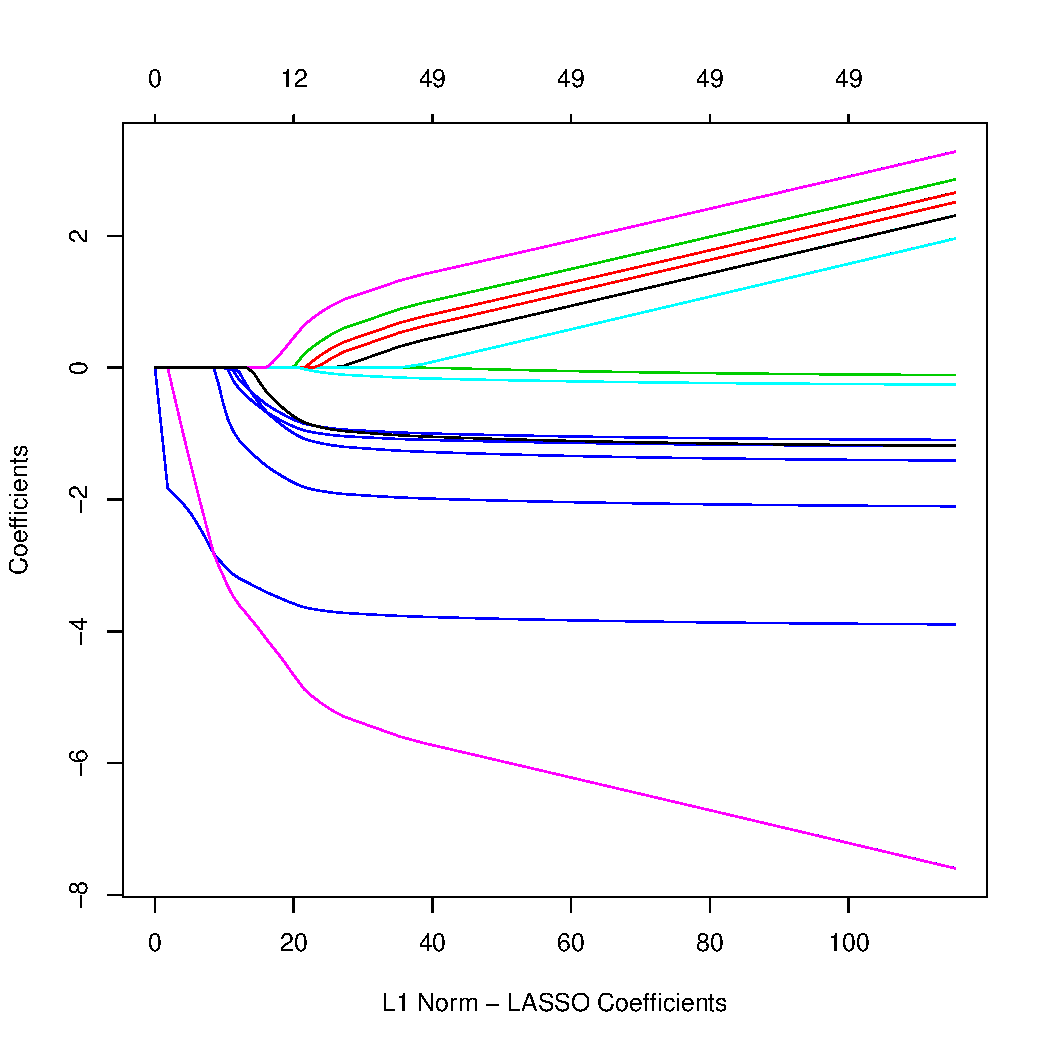
\includegraphics[height=2.0in,width=2.0in]{LassoModel1}
  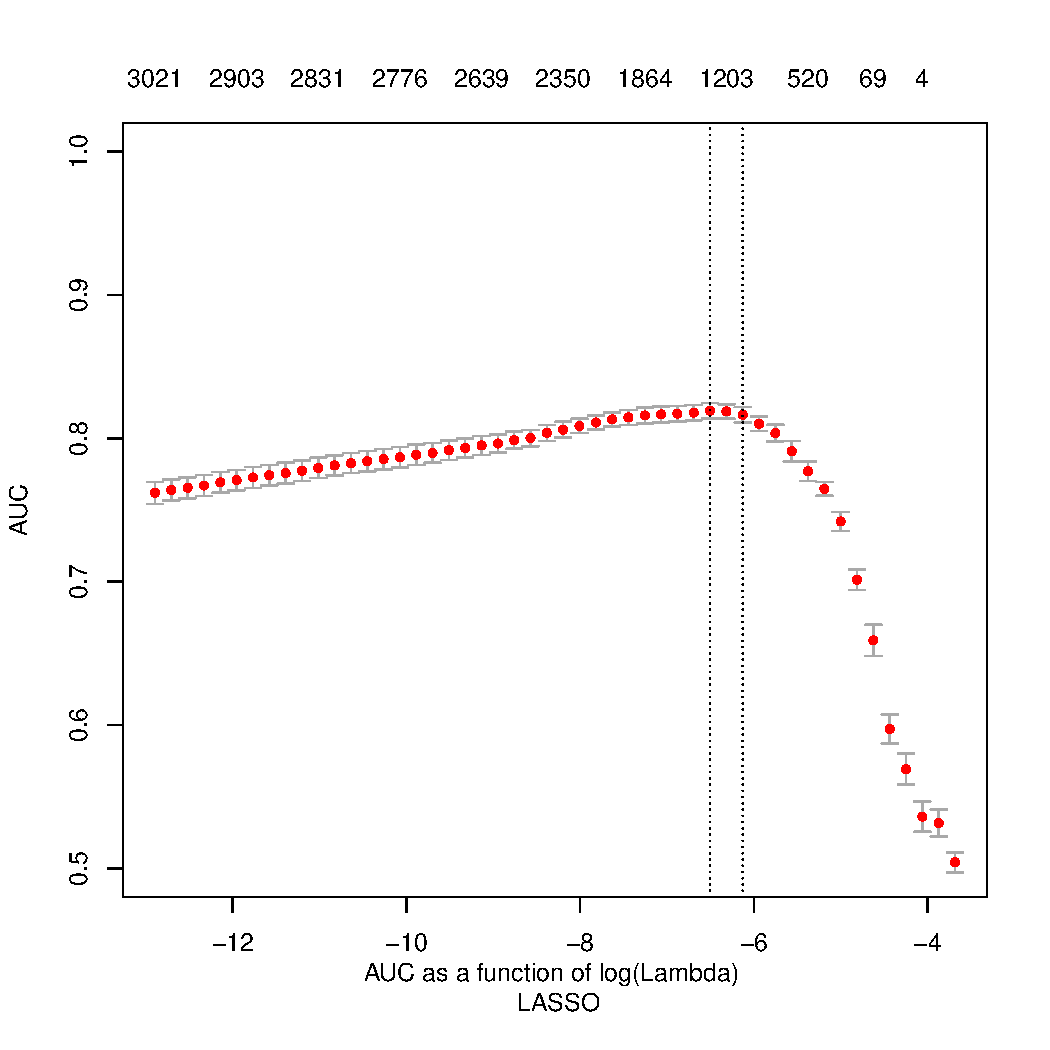
\includegraphics[height=2.0in,width=2.0in]{LassoModel2}
}
\end{frame}

\subsection{Amazon Data: Ridge Model}
\begin{frame}
\frametitle{Ridge Model Performance}
\framebox{
  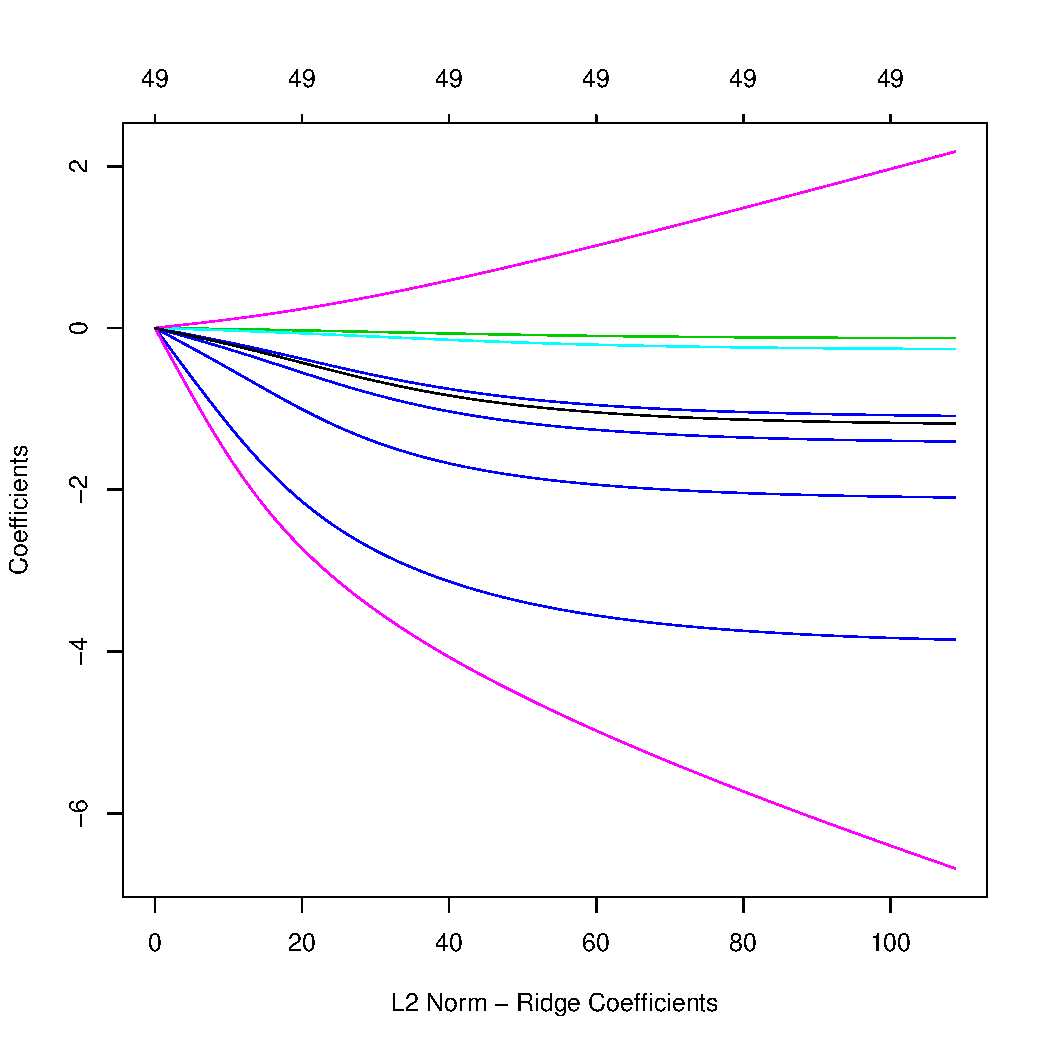
\includegraphics[height=2.0in,width=2.0in]{RidgeModel1}
  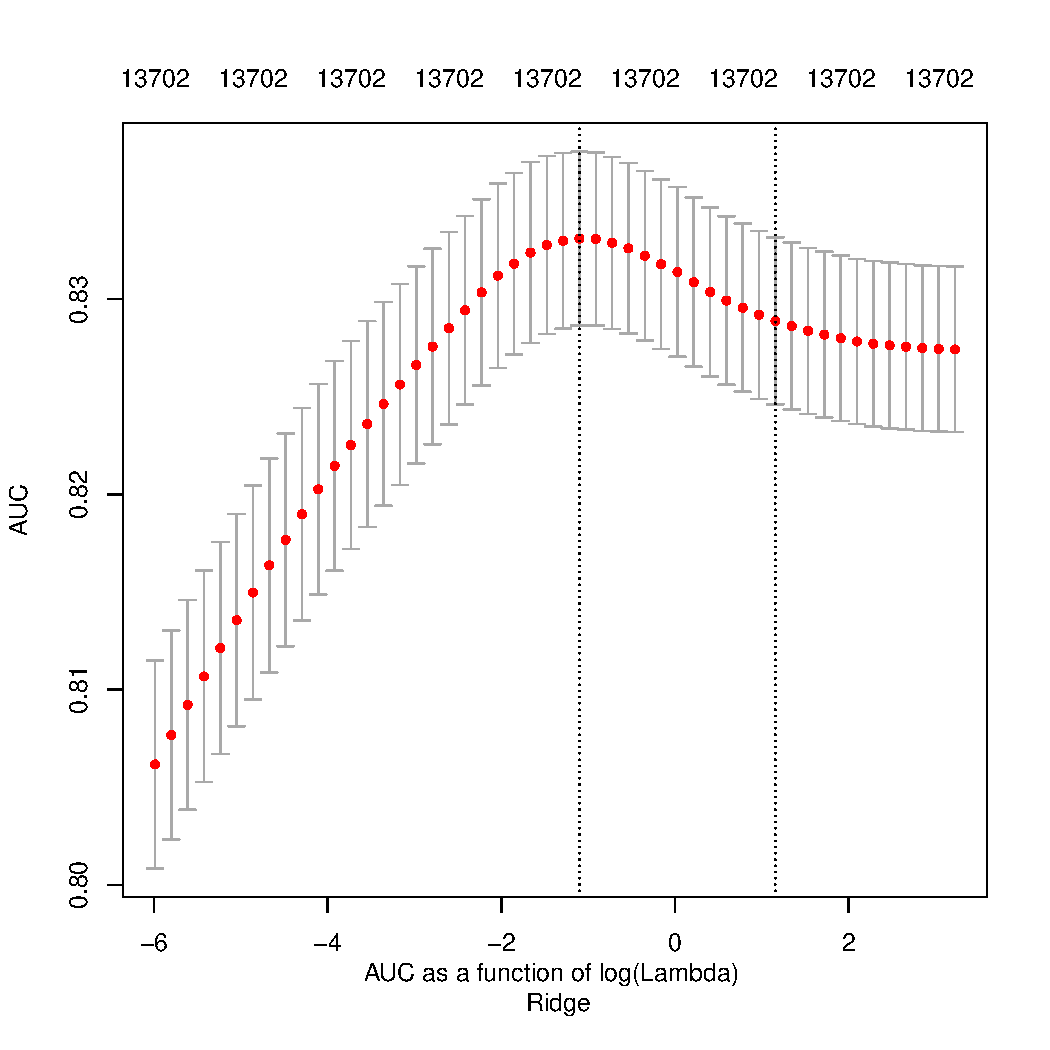
\includegraphics[height=2.0in,width=2.0in]{RidgeModel2}
}
\end{frame}


\subsection{Amazon Data: Performance}
\begin{frame}
\frametitle{Comparison of Ridge, LASSO, and OLS}
\framebox{
  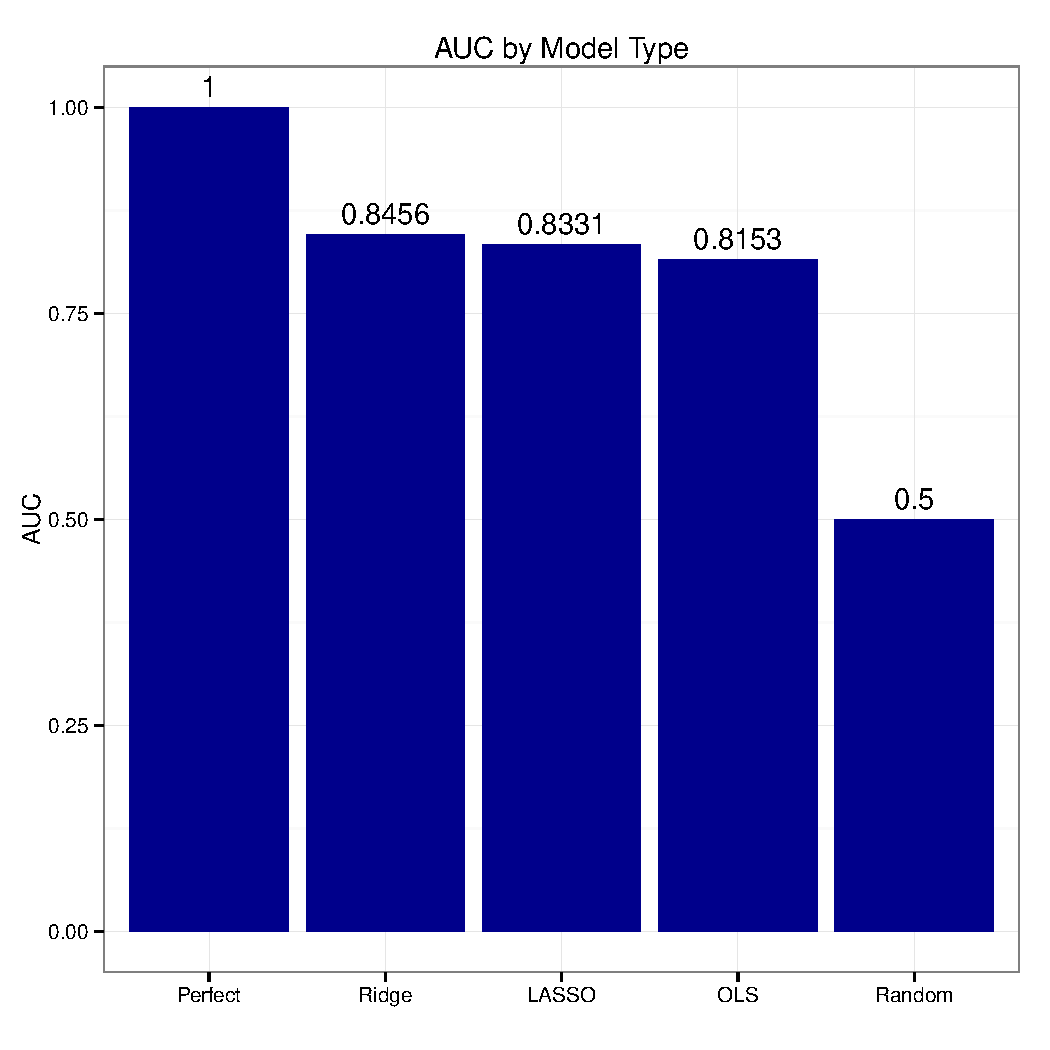
\includegraphics[height=2.0in,width=2.0in]{ModelPerformance}
  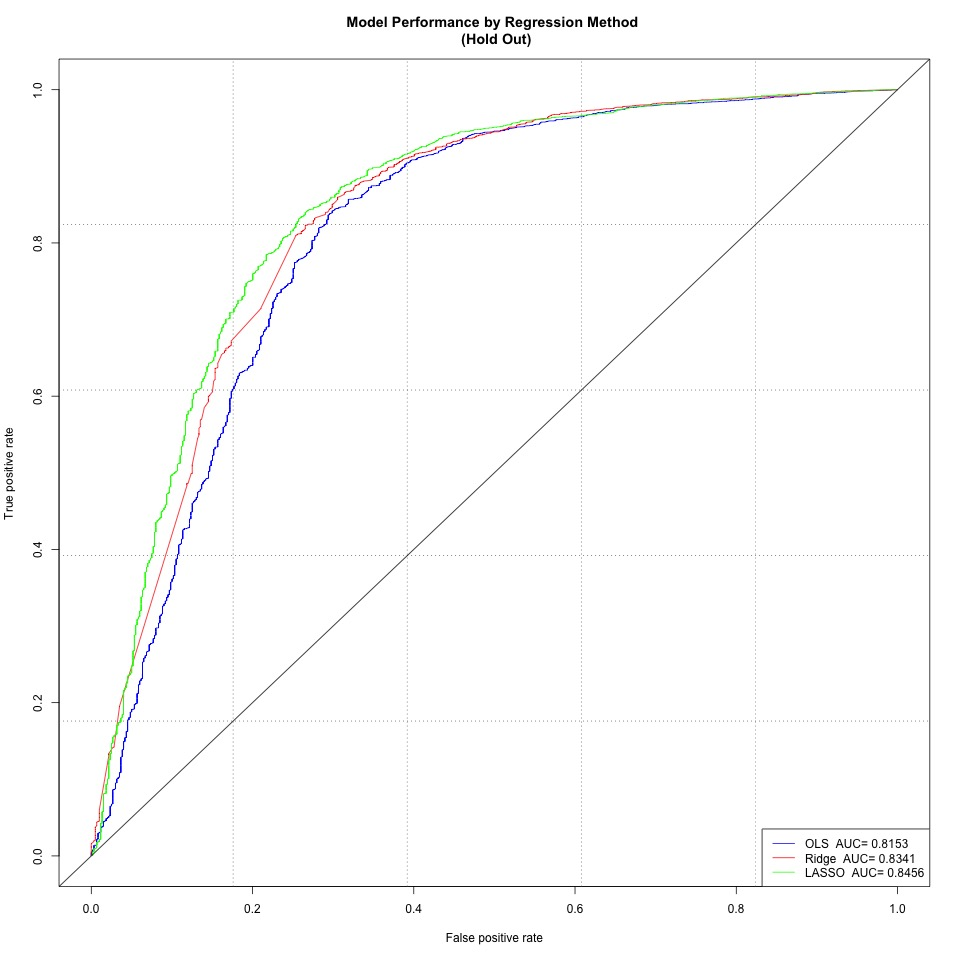
\includegraphics[height=2.0in,width=2.0in]{AUCbyModel}
}
\end{frame}

\section{Some Resources}
\begin{frame}
\frametitle{Useful Links below}
Thank you.
\begin{itemize}
\item<1-> \href{mailto:fja2114@columbia.edu}{My Email (Not as Useful)}
\item<2-> \href{https://github.com/franciscojavierarceo/Amazon/blob/master/RegularizedRegressionExample.R}{GitHub (Moderately Useful)}
\item<3-> \href{http://cran.r-project.org/web/packages/glmnet/glmnet.pdf}{GLMNET in R (Very Useful)}
\item<4-> \href{http://scikit-learn.org/0.10/auto_examples/linear_model/lasso_and_elasticnet.html}{SKLearn (Also Very Useful)}
\item<5-> \href{http://statweb.stanford.edu/~tibs/lasso/lasso.pdf}{Original LASSO Publication (REALLY Useful)}
\item<6-> \href{http://math.arizona.edu/~hzhang/math574m/Read/Ridge.pdf}{Original Ridge Publication (Somewhat useful)}
\item<7-> \href{http://statweb.stanford.edu/~owen/courses/305/Rudyregularization.pdf}{Slides from Stanford (Most Useful)}
\item<8-> \href{http://arxiv.org/pdf/1306.5505v3.pdf}{Sweet paper on asymptotic properties of Ridge and LASSO}
\end{itemize}
\end{frame}
\end{document}